\documentclass{beamer}
\mode<presentation> {
\usepackage{color}
\definecolor{bottomcolour}{rgb}{0.21,0.11,0.21}
\definecolor{middlecolour}{rgb}{0.21,0.11,0.21}
\setbeamercolor{structure}{fg=white}
\setbeamertemplate{frametitle}[default]%[center]
\setbeamercolor{normal text}{bg=black, fg=white}
\setbeamertemplate{background canvas}[vertical shading]
[bottom=bottomcolour, middle=middlecolour, top=black]
\setbeamertemplate{items}[circle]
\setbeamertemplate{navigation symbols}{} %no nav symbols
\setbeamercolor{block title}{use=structure,fg=white,bg=structure.fg!50!red!50!blue!100!green}
\setbeamercolor{block body}{parent=normal text,use=block title,bg=block title.bg!5!white!10!bg,fg=white}
\setbeamertemplate{navigation symbols}{}
}
\usepackage{graphicx} 
\usepackage{booktabs} 
\usepackage[utf8]{inputenc}  
\usepackage{geometry}     
\usepackage{eurosym}
\usepackage{verbatim}
\usepackage{ragged2e}
\justifying

%%%%%%%%%%%%%%%%%%%%%%%%%%%%%%%%%%%%%%%%%%%%%%%%%%%%%%%%%%%%%%%%
%% ccBeamer 0.1, 2007-07-02                                   %%
%% Written by Sebastian Pipping <webmaster@hartwork.org>      %%
%% ---------------------------------------------------------- %%
%% Licensed under Creative Commons Attribution-ShareAlike 3.0 %%
%% http://creativecommons.org/licenses/by-sa/3.0/             %%
%%%%%%%%%%%%%%%%%%%%%%%%%%%%%%%%%%%%%%%%%%%%%%%%%%%%%%%%%%%%%%%%


%% Images
\newcommand{\CcImageBy}[1]{%
	
\includegraphics[scale=#1]{creative_commons/cc_by_30.pdf}%
}
\newcommand{\CcImageCc}[1]{%
	
\includegraphics[scale=#1]{creative_commons/cc_cc_30.pdf}%
}
\newcommand{\CcImageDevNations}[1]{%
	
\includegraphics[scale=#1]{creative_commons/cc_dev_nations_30.pdf}%
}
\newcommand{\CcImageNc}[1]{%
	
\includegraphics[scale=#1]{creative_commons/cc_nc_30.pdf}%
}
\newcommand{\CcImageNd}[1]{%
	
\includegraphics[scale=#1]{creative_commons/cc_nd_30.pdf}%
}
\newcommand{\CcImagePd}[1]{%
	
\includegraphics[scale=#1]{creative_commons/cc_pd_30.pdf}%
}
\newcommand{\CcImageSa}[1]{%
	
\includegraphics[scale=#1]{creative_commons/cc_sa_30.pdf}%
}
\newcommand{\CcImageSampling}[1]{%
	
\includegraphics[scale=#1]{creative_commons/cc_sampling_30.pdf}%
}
\newcommand{\CcImageSamplingPlus}[1]{%
	
\includegraphics[scale=#1]{creative_commons/cc_sampling_plus_30.pdf}%
}


%% Groups
\newcommand{\CcGroupBy}[1]{% zoom
	\CcImageBy{#1}%
}
\newcommand{\CcGroupByNc}[2]{% zoom, gap
	\CcImageBy{#1}\hspace*{#2}\CcImageNc{#1}%
}
\newcommand{\CcGroupByNcNd}[2]{% zoom, gap
	\CcImageBy{#1}\hspace*{#2}\CcImageNc{#1}\hspace*{#2}\CcImageNd{#1}%
}
\newcommand{\CcGroupByNcSa}[2]{% zoom, gap
	\CcImageBy{#1}\hspace*{#2}\CcImageNc{#1}\hspace*{#2}\CcImageSa{#1}%
}
\newcommand{\CcGroupByNd}[2]{% zoom, gap
	\CcImageBy{#1}\hspace*{#2}\CcImageNd{#1}%
}
\newcommand{\CcGroupBySa}[2]{% zoom, gap
	\CcImageBy{#1}\hspace*{#2}\CcImageSa{#1}%
}
\newcommand{\CcGroupDevNations}[1]{% zoom
	\CcImageDevNations{#1}%
}
\newcommand{\CcGroupNcSampling}[2]{% zoom, gap
	\CcImageNc{#1}\hspace*{#2}\CcImageSampling{#1}%
}
\newcommand{\CcGroupPd}[1]{% zoom
	\CcImagePd{#1}%
}
\newcommand{\CcGroupSampling}[1]{% zoom
	\CcImageSampling{#1}%
}
\newcommand{\CcGroupSamplingPlus}[1]{% zoom
	\CcImageSamplingPlus{#1}%
}


%% Text
\newcommand{\CcLongnameBy}{Attribution}
\newcommand{\CcLongnameByNc}{Attribution-NonCommercial}
\newcommand{\CcLongnameByNcNd}{Attribution-NoDerivs}
\newcommand{\CcLongnameByNcSa}{Attribution-NonCommercial-ShareAlike}
\newcommand{\CcLongnameByNd}{Attribution-NoDerivs}
\newcommand{\CcLongnameBySa}{Attribution-ShareAlike}

\newcommand{\CcNote}[1]{% longname
	This work is licensed under the \textit{Creative Commons #1 3.0 License}.%
}

\title[Les réseaux sociaux]{Les réseaux sociaux} 
\author{Genma}
\begin{document}
%% Titlepage
\begin{frame}
	\titlepage
	\vfill
	\begin{center}
		\CcGroupByNcSa{0.83}{0.95ex}\\[2.5ex]
		{\tiny\CcNote{\CcLongnameByNcSa}}
		\vspace*{-2.5ex}
	\end{center}
\end{frame}

%----------------------------------------------------------------------------------------
\begin{frame}
\begin{center}
\Huge{Introduction}
\end{center}
\end{frame}

%----------------------------------------------------------------------------------------
\begin{frame}
\frametitle{Comprendre les réseaux sociaux?}

\justifying{
Internet comment ça marche, qu'est ce que le web 2.0? 
\\~\\Les réseaux sociaux : quels sont les principes, les principaux sites, les avantages et les risques à les utiliser? 
\\~\\Qu'est ce que l'e-réputation ou l'identité numérique?}
\end{frame}


%----------------------------------------------------------------------------------------
\begin{frame}
\frametitle{Qui suis-je?}

\begin{block}{Jérôme...}
\begin{itemize}
\justifying{
\item C'est mon prénom civil.
\item Cette identité numérique existe, mais dans le cadre de la gestion de mon e-reputation.
}
\end{itemize}
\justifying{Ne pas être présent en ligne est \emph{presque} suspect...}
\end{block}

\begin{block}{mais surtout Genma!}
\begin{itemize}
\justifying{
\item Auteur du blog \emph{le Blog de Genma} \url{http://genma.free.fr} depuis 2004
\item Identité numérique publique, assez forte (Réseaux sociaux) et \emph{cohérente}.
\item Identité de type \emph{pseudonymat} et non relié à mon identité civile.
}
\end{itemize}
\end{block}
\end{frame}
%----------------------------------------------------------------------------------------
\begin{frame}
\begin{center}
\Huge{L'évolution d'Internet\\en quelques mots...}
\end{center}
\end{frame}

%----------------------------------------------------------------------------------------
\begin{frame}
\frametitle{Internet, un réseau de réseau}
\begin{itemize}
\justifying{
\item Internet c'est un réseau de réseau d'ordinateurs connectés entre eux.
\item Il y a d'un côté les serveurs, des gros ordinateurs, sur lesquels il y a des sites Internet.
\item Et de l'autre, il y a "nous", avec notre PC, notre tablette, notre smartphone...
}
\end{itemize}
\end{frame}

%----------------------------------------------------------------------------------------
\begin{frame}
\frametitle{Internet : 3 phases}
\begin{block}{Web 1.0}
\justifying{
Des images fixes, des pages fixes, des forums...
\begin{itemize}
\justifying{
\item L'usage d'un pseudonyme était courant voir une évidence.
}
\end{itemize}
}
\end{block}

\begin{block}{Web 2.0}
\begin{itemize}
\justifying{
\item Les blogs, la possibilité de laisser des commentaires
\item Apparition des wikis (Wikipedia)
}
\end{itemize}
\end{block}

\begin{block}{Web 2.5}
\justifying{
Apparition de Facebook, Twitter....
}
\begin{itemize}
\justifying{
\item L'usage de son identité civile devient obligatoire...
}
\end{itemize}
\end{block}
\end{frame}

%----------------------------------------------------------------------------------------
\begin{frame}
\begin{center}
\Huge{Les réseaux sociaux}\\~\\
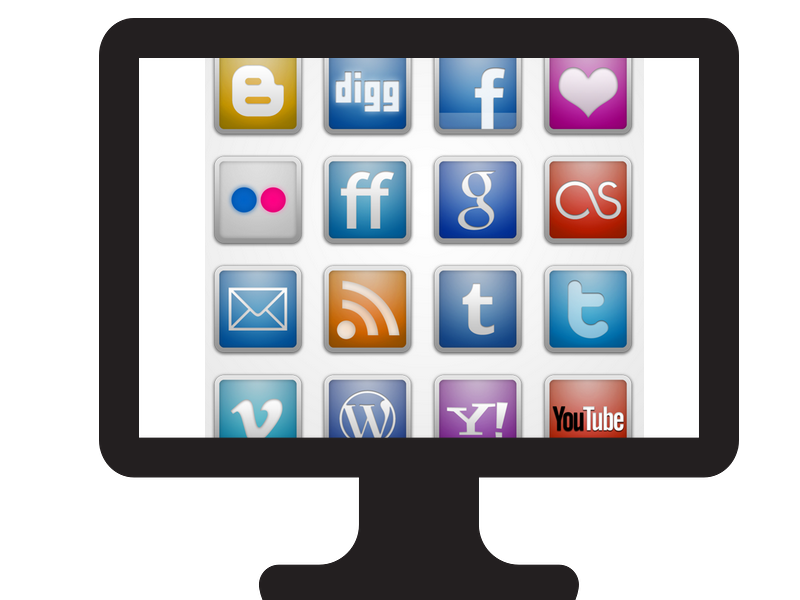
\includegraphics[scale=0.4] {./images/Resaux_sociaux.png} 
\end{center}
\end{frame}

%----------------------------------------------------------------------------------------
\begin{frame}
\frametitle{Définition des réseaux sociaux}

\begin{block}{Proposition d'une définition très large et personnelle}
\justifying{
\emph{Un réseau social est un site Internet sur lequel, une fois inscrit, il est possible de se lier à d'autres inscrits, pour suivre ou leur diffuser de l'information. Les inscrits étant des personnes physiques ou morales}
}
\end{block}
\end{frame}

%----------------------------------------------------------------------------------------
\begin{frame}
\begin{center}
\Huge{Présentation de quelques réseaux dit \emph{sociaux}\\
parmi les plus \emph{connus}}
\end{center}
\end{frame}

%----------------------------------------------------------------------------------------
\begin{frame}
\frametitle{
\includegraphics[scale=0.2] {./images/twitter_logo.jpg}~ Twitter}
\begin{center}
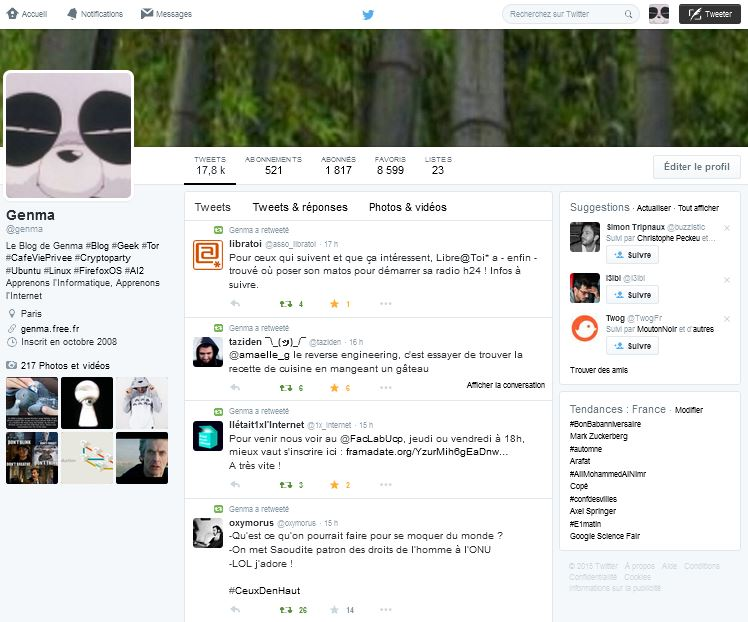
\includegraphics[scale=0.6] {./images/twitter_capture.jpg} 
\end{center}
\end{frame}

\begin{frame}
\frametitle{
\includegraphics[scale=0.2] {./images/twitter_logo.jpg} ~Twitter}
\begin{block}{Présentation}
\justifying{
Outil de \emph{microblogage}
\begin{itemize}
\item Messages limités à 140 caractères
\item Utilisation des \#hastags
\end{itemize}
}
\end{block}

\begin{block}{Conseils}
\begin{itemize}
\justifying{
\item Choisir les personnes que l'on suit
\item Remplir sa biographie
\item Utiliser les \#hastag pour filtrer
\item Ne pas hésiter à bloquer des utilisateurs
\item Comprendre les codes et usages
}
\end{itemize}
\end{block}
\end{frame}

%----------------------------------------------------------------------------------------
\begin{frame}
\frametitle{
\includegraphics[scale=0.15] {./images/facebook_logo.jpg} ~ Facebook}
\begin{block}{Présentation}
\begin{itemize}
\justifying{
\item Un réseau qui comprend plus d'un Milliard de personnes
\item \emph{Tout le monde} est sur Facebook
\item Permet de poster des photos, de commenter, de voir des vidéos...
}
\end{itemize}
\end{block}

\begin{block}{Conseils}
\begin{itemize}
\justifying{
\item Ne pas liker n'importe quoi
\item Ne pas prendre n'importe qui en amis
}
\end{itemize}
\end{block}

\end{frame}

%----------------------------------------------------------------------------------------
\begin{frame}
\frametitle{
\includegraphics[scale=0.15] {./images/linkedin_logo.jpg} ~ Linkedin / Viadeo}
\begin{center}
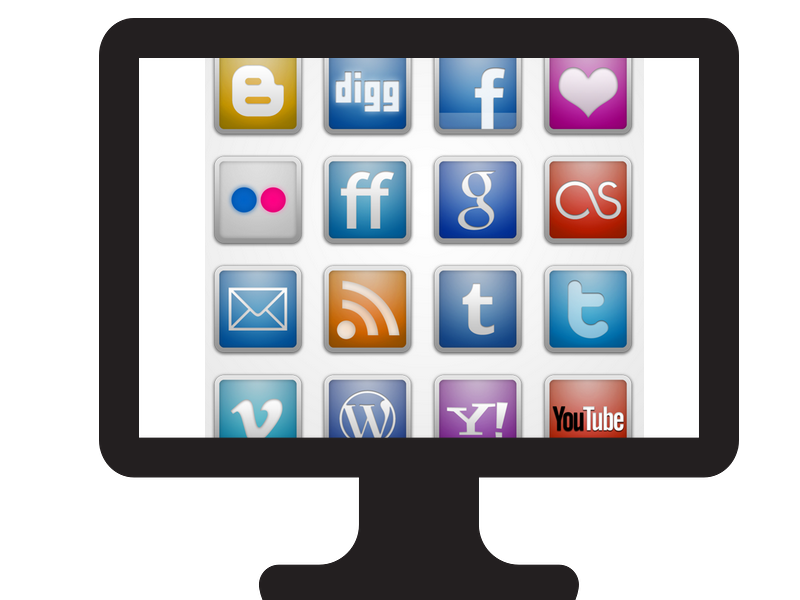
\includegraphics[scale=0.4] {./images/Resaux_sociaux.png} 
\end{center}
\end{frame}

\begin{frame}
\frametitle{
\includegraphics[scale=0.15] {./images/linkedin_logo.jpg} ~ Linkedin / Viadeo}
\begin{block}{Présentation}
\justifying{ 
Destiné à du \emph{réseautage} professionnel.
}
\begin{itemize}
\justifying{
\item Permet de garder contact avec ses collègues
\item Permet de prospecter pour un nouvel emploi
}
\end{itemize}
\justifying{ C'est une sorte de CV en ligne.}
\end{block}
\end{frame}

%----------------------------------------------------------------------------------------
\begin{frame}
\begin{center}
\Huge{Autres réseaux sociaux célèbres}
\end{center}
\end{frame}

%----------------------------------------------------------------------------------------
\begin{frame}
\frametitle{Pinterest}
\justifying{Concept : partage de collections de photos }
\begin{center}
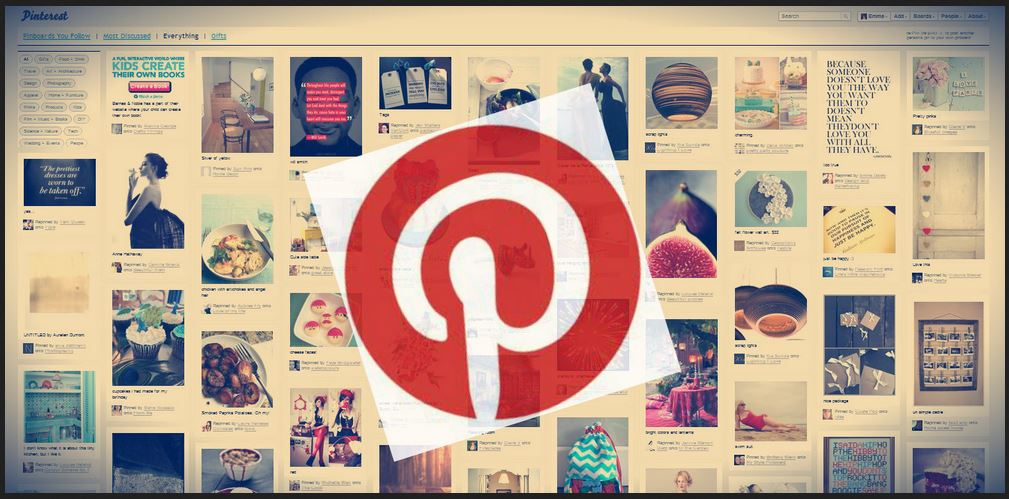
\includegraphics[scale=0.6] {./images/pinterest.jpg} 
\end{center}
\end{frame}

\begin{frame}
\frametitle{GooglePlus}
\justifying{Concept : le réseau social par Google}
\begin{center}
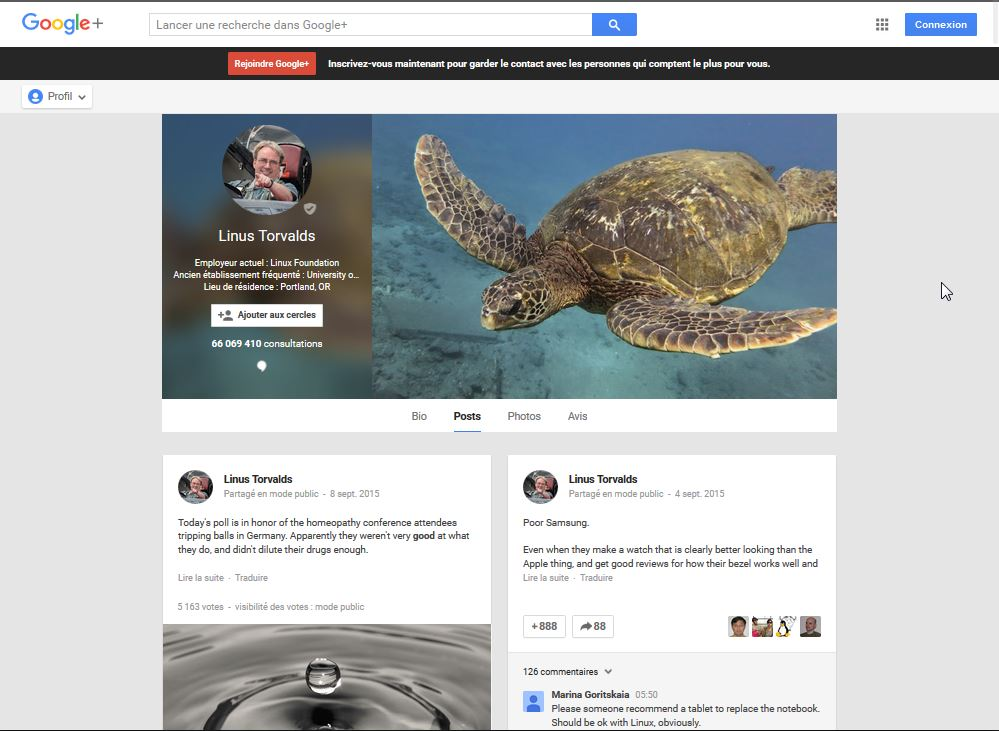
\includegraphics[scale=0.4] {./images/googleplus.jpg} 
\end{center}
\end{frame}

\begin{frame}
\frametitle{Kickstarter et les plateformes de crowdfounding}
\justifying{Concept : le financement participatif de projets}
\begin{center}
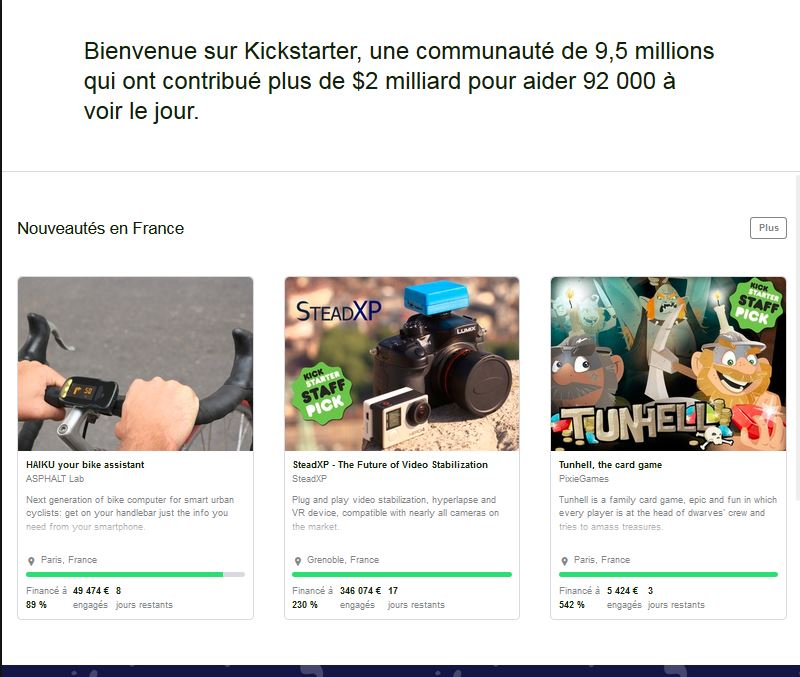
\includegraphics[scale=0.5] {./images/kickstarter.jpg} 
\end{center}
\end{frame}

\begin{frame}
\frametitle{Vine}
\justifying{Concept : Vine est une application de Twitter qui héberge de courtes vidéos de 6 secondes qui tournent en boucle }\begin{center}

\includegraphics[scale=0.4] {./images/vine.jpg} 
\end{center}
\end{frame}

\begin{frame}
\frametitle{Instagram}
\justifying{Concept : partage de photographies retouchées avec des filtres (sépia...) }
\begin{center}
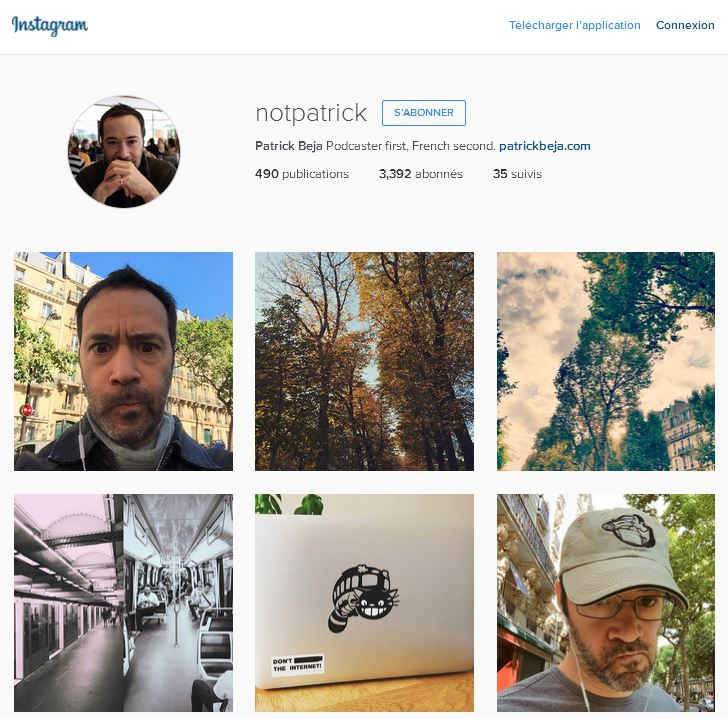
\includegraphics[scale=0.5] {./images/instagram.jpg} 
\end{center}
\end{frame}

\begin{frame}
\frametitle{tumblr}
\justifying{Concept : un blog d'images (souvent thématiques, drôle...)}
\begin{center}
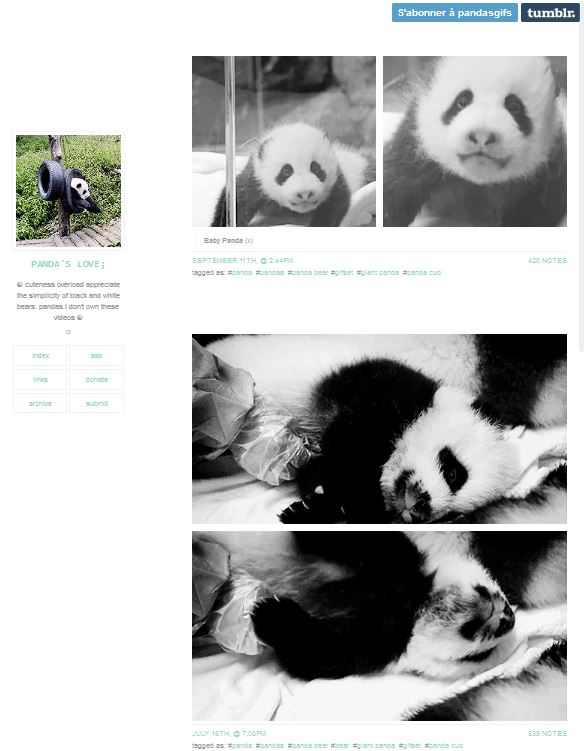
\includegraphics[scale=0.4] {./images/tumblr.jpg} 
\end{center}
\end{frame}

%----------------------------------------------------------------------------------------
\begin{frame}
\begin{center}
\Huge{Et tous les autres... \\Il en apparait et disparait régulièrement.}
\end{center}
\end{frame}

%----------------------------------------------------------------------------------------
\begin{frame}
\begin{center}
\Huge{Etre présent en ligne}
\end{center}
\end{frame}

%-----------------------------------------------
\begin{frame}
\frametitle{Les questions à de poser sur sa présence en ligne}

\justifying{
On tape mes "noms prénoms" dans un moteur de recherche :
\begin{itemize}
\item Quelles informations trouve-t-on sur moi?
\item Quelle image je donne de moi?
\item Suis en capacité d'assumer tout ce que l'on trouve sur moi? De le justifier?
\item Est-ce qu'il y a des choses que je voudrais cacher?
\item Que je regrette?
\end{itemize}
}
\end{frame}

%-----------------------------------------------
\begin{frame}
\frametitle{Les données publiques et personnelles}

\justifying{
La quasi totalité des informations que l'on trouve sur nous, ce sont des informations que NOUS avons mis en ligne (via les réseaux sociaux par exemple).
}

\end{frame}

%----------------------------------------------------------------------------------------
\begin{frame}
\frametitle{Adage}
\begin{block}{Les paroles s'envolent, les écrits restent}
\begin{itemize}
\justifying{
\item Cet adage est encore plus vrai avec Internet.
\item Il faut partir du principe que ce que l'on dit sera toujours accessible, même des années après.
\item Tout ce qui est sur Internet est public ou le sera (même si c'est "privé". Les conditions d'utilisation évoluent. Cf. Facebook).
\item Il ne faut donc pas abuser de la liberté d'expression et rester respectueux des lois en vigueurs.
}
\end{itemize}
\end{block}
\end{frame}

%----------------------------------------------------------------------------------------
\begin{frame}
\frametitle{La netiquette}

\begin{block}{Définition}
\justifying{
La nétiquette est une règle informelle, puis une charte qui définit les règles de conduite et de politesse recommandées sur les premiers médias de communication mis à disposition par Internet. Il s'agit de tentatives de formalisation d'un certain contrat social pour l'Internet.
}
\end{block}
\justifying{
En résumé ce sont les règles de savoir vivre et de respect que l'on devrait tou-te-s avoir sur Internet.}
\end{frame}


%----------------------------------------------------------------------------------------
\begin{frame}
\begin{center}
\Huge{Les \emph{risques} des réseaux sociaux}
\end{center}
\end{frame}

%----------------------------------------------------------------------------------------
\begin{frame}
\frametitle{Messages interdits}

\begin{block}{Les Hommes restent des Hommes...} 
\justifying{
Les messages de type terroristes, nazis, pédophiles, racistes, antisémites, homophobes... tombent sous le coup de la loi.
Ne pas les diffuser pour les \emph{dénoncer}.
}
\end{block}
Il faut les signaler \url{http://internet-signalement.gouv.fr}
\end{frame}

%----------------------------------------------------------------------------------------
\begin{frame}
\frametitle{Le syndrôme téléréalité}

\begin{block}{Ne pas vouloir être \emph{une star}}
\begin{itemize}
\justifying{
\item Ne pas chercher à avoir le plus grand nombre de personnes ;
\item Ne pas exposer sa vie que ce soit avec des photos, vidéos ou des messages.
}
\end{itemize}
\end{block}
Rappel : ce n'est pas parce qu'on est derrière un écran qu'on doit faire n'importe quoi.
\end{frame}

%----------------------------------------------------------------------------------------
\begin{frame}
\frametitle{Réserver les comptes}

\begin{block}{Ne pas s'inscrire partout}
\begin{itemize}
\justifying{
\item Ca ne sert à rien.
\item C'est une \emph{Perte de temps}.
\item Si ce n'est pour "réserver/bloquer" le compte, pour éviter une usurpation par quelqu'un d'autre.
}
\end{itemize}
\end{block}
\end{frame}

%----------------------------------------------------------------------------------------
\begin{frame}
\frametitle{Droit à l'oubli}

\begin{block}{Législation}
\justifying{Par un arrêt du 13 mai 2014 , la CJUE a reconnu le droit pour les particuliers de demander à faire supprimer des résultats de recherche Google les liens vers les pages mentionnant des données personnelles les concernant. 
\\~\\
C'est ce que l'on appelle \emph{le droit à l'oubli}.
}
\end{block}
 \url{https://support.google.com/legal/contact/lr_eudpa?product=websearch&hl=fr}
\end{frame}

%----------------------------------------------------------------------------------------
\begin{frame}
\frametitle{Les réseaux sociaux et les enfants}

\begin{block}{Quelques conseils}
\begin{itemize}
\justifying{
\item Pas de compte avant 13 ans
\item Le sensibiliser aux \emph{dangers} d'Internet
\item Leur donner un regard critique sur ce qu'ils lisent, transmettent comme information
\item Les sensibiliser à l'usage d'un pseudonyme
}
\end{itemize}
\end{block}
\end{frame}

%----------------------------------------------------------------------------------------
\begin{frame}
\frametitle{Les risques des réseaux sociaux}

\begin{block}{Centralisation des données}
\justifying{
En un seul endroit (Facebook par exemple), il y a énormément d'informations personnelles qui sont cumulées.
\begin{itemize}
\item Ces données peuvent être accessibles de n'importe qui, si le compte est \emph{mal configuré}.
\item Risque d'attaque de type \emph{social enginering}.
\item Risque de cambriolage....
\end{itemize}
}
\end{block}

\begin{block}{Si c'est gratuit, c'est vous le produit}
\justifying{
\begin{itemize}
\item Ces données sont revendues et exploitées.
\end{itemize}
}
\end{block}
\justifying{
D'où l'importance de se créer une identité numérique sous pseudonyme, sur laquelle on a un contrôle \emph{relatif}.
}

\end{frame}
%----------------------------------------------------------------------------------------
\begin{frame}
\frametitle{Sécuriser ses comptes}

\begin{block}{Un bon mot de passe...}
\justifying{
Est idéalement une phrase de passe.
\begin{itemize}
\item "LaLuneRougeEtLeSoleilVert" est un meilleur mot de passe que R0x0r75.
\item Plusieurs mots du dictionnaires sans liens.
\end{itemize}
}
Point important : \textbf{Un mot de passe différent par compte}.
\end{block}

\begin{block}{Double authentification}
\justifying{
\begin{itemize}
\item On reçoit un code à usage unique sur son téléphone.
\end{itemize}
}
\end{block}
\end{frame}

%----------------------------------------------------------------------------------------
\begin{frame}
\begin{center}
\Huge{Les points positifs \\ des réseaux sociaux}
\end{center}
\end{frame}

%----------------------------------------------------------------------------------------
\begin{frame}
\frametitle{Les points positifs des réseaux sociaux}

\begin{block}{Discuter}
\justifying{
\begin{itemize}
\item Discussion avec des amis
\item Permettent de garder contact
\item Permettent de découvrir de nouvelles personnes
\end{itemize}
}
\end{block}

\begin{block}{S'informer}
\justifying{
\begin{itemize}
\item Source d'information alternative 
\item Veille technologique
\end{itemize}
}
\end{block}
\end{frame}
%----------------------------------------------------------------------------------------
\begin{frame}
\begin{center}
\Huge{Conclusion}
\end{center}
\end{frame}

%-----------------------------------------------
\begin{frame}
\frametitle{Conclusion}

Il faut gérer son image comme une marque (on appelle ça le \emph{personnal branding}).
\\~\\
Il faut prendre consience des risques pour la vie privée.

\end{frame}

%----------------------------------------------------------------------------------------
\begin{frame}
\begin{center}
\Huge{Merci de votre attention. \\~\\ Place aux questions.}
\end{center}
\end{frame}

\end{document}
